\documentclass[a4paper]{scrartcl}
\pagestyle{plain}
\usepackage{a4wide}
\usepackage{tikz}
\usepackage{enumerate}
\usepackage{listings}
\usepackage[colorlinks=true,linkcolor=black,a4paper=true]{hyperref}
\usetikzlibrary{calc}
\usetikzlibrary{matrix}
\usetikzlibrary{automata}
\usetikzlibrary{decorations.pathreplacing}
\usetikzlibrary{positioning}
\usepackage{dsfont}
\usepackage{amsmath, amsthm, amssymb}
\usepackage{ifxetex}
\usepackage{color}
\usepackage{scrpage2}

\ifxetex
 \usepackage[EU1]{fontenc}
 \usepackage[no-math]{fontspec}
 \usepackage{lmodern}
 \usepackage{xunicode}
 \defaultfontfeatures{Scale=MatchLowercase, Mapping=tex-text}
 \setsansfont{Latin Modern Sans}
 \setmonofont[SmallCapsFont={Latin Modern Mono Caps}]{Latin Modern Mono Light}
\else
 \usepackage[utf8]{inputenc}
\fi

% Pretty captions!
\usepackage{caption}
\DeclareCaptionFont{white}{\color{white}}
\DeclareCaptionFormat{listing}{\colorbox{gray}{\parbox{0.98\linewidth}{#1#2#3}}}
\captionsetup[lstlisting]{format=listing,labelfont=white,textfont=white}

% Pretty page headings!
\pagestyle{scrheadings}
\clearscrheadings
\clearscrplain
\setfootwidth{head}
\ofoot{\pagemark}

\makeatletter
% Different format for headings
\def\section{\@startsection{section}{1}%
  \z@{.7\baselineskip\@plus\baselineskip}{.5\baselineskip}%
  {\normalfont\large\scshape\centering}}
% This does spacing around caption.
\setlength{\abovecaptionskip}{0.5em}
\setlength{\belowcaptionskip}{0.5em}
% This does justification (left) of caption.
\long\def\@makecaption#1#2{%
  \vskip\abovecaptionskip
  \sbox\@tempboxa{#2}%
  \ifdim \wd\@tempboxa >\hsize
    #2\par
  \else
    \global \@minipagefalse
    \hb@xt@\hsize{\box\@tempboxa\hfill}%
  \fi
  \vskip\belowcaptionskip}
\makeatother

\title{Komplexität von Algorithmen\\
       Sommersemester 2011 \\
       \small Lösungen zu den Übungsaufgaben}
\author{\LaTeX-Version von Christoph Rauch\\ FAU Erlangen-Nürnberg}

\begin{document}
\maketitle
\tableofcontents
\section*{Aufgabe 4 - Fibonacci}
\addcontentsline{toc}{subsection}{Aufgabe 4 - Fibonacci}
\begin{paragraph}{a)}
  zu zeigen:
  \[ f_n = \frac{\Phi^n - \hat \Phi^n}{\sqrt{5}} \quad n \geq 0 \]
  \begin{itemize}
    \item Induktionsanfang:
    \begin{itemize}
      \item[$n = 0$]
        \[ f_0 = \frac{\Phi^0 - \hat \Phi^0}{\sqrt{5}} 
               = \frac{1 - 1}{\sqrt{5}} = 0 \]
      \item[$n = 1$]
        \[ f_1 = \frac{\Phi - \hat \Phi}{\sqrt{5}} 
               = \frac{1 + \sqrt{5} - 1 + \sqrt{5}}{2 \sqrt{5}} = 1 \]
    \end{itemize}
    \item Induktionsvoraussetzung: Die Behauptung gelte für $n$.
    \item Induktionsschritt: $n \rightarrow n + 1$
    
    Da $\Phi$ und $\hat \Phi$ die beiden Lösungen der quadratischen Gleichung
    $x^2 - x - 1 = 0$ sind, gilt offensichtlich $\Phi + 1 = \Phi^2$ sowie
    $\hat \Phi + 1 = \hat \Phi^2$.
%    \[ \Phi + 1 = \frac{3 + \sqrt{5}}{2} = \frac{6 + 2 \sqrt{5}}{4} 
%                = \frac{1 + s \sqrt{5} + 5}{4} = (\frac{1 + \sqrt{5}}{2})^2 
%                = \Phi^2 \]
%    analog gilt:
%    \[ \hat \Phi + 1 = \hat \Phi^2 \]
    
    Damit folgt:
    \[ f_{n+1} = f_n + f_{n-1} \overset{IV}{=} \frac{\Phi^n - \hat
       \Phi^n}{\sqrt{5}} + \frac{\Phi^{n-1} - \hat \Phi^{n-1}}{\sqrt{5}} = \]
    \[ = \frac{(\Phi^n + \Phi^{n-1}) - (\hat \Phi^n + \hat \Phi^{n-1})}{\sqrt{5}}
       = \frac{(\Phi^{n-1} \cdot \Phi + \Phi^{n-1}) - 
         (\hat \Phi^{n-1} \cdot \hat \Phi + \hat \Phi^{n-1})}{\sqrt{5}} = \]
    \[ = \frac{(\Phi^{n-1} (\Phi + 1)) - (\hat \Phi^{n-1} (\hat \Phi + 1))}{\sqrt{5}} 
       = \frac{\Phi^{n-1} \Phi^2 - \hat \Phi^{n-1} \hat \Phi^2}{\sqrt{5}} = \]
    \[ = \frac{\Phi^{n+1} - \hat \Phi^{n+1}}{\sqrt{5}} \]
    $\hfill \square$
  \end{itemize}
\end{paragraph}
\begin{paragraph}{b)}
  zu zeigen:
  \[ f_{n+1} f_{n-1} - f_n^2 = (-1)^n \quad n \geq 1 \]
  \begin{itemize}
    \item Induktionsanfang:
    \begin{itemize}
      \item[$n = 1$] \[ f_2f_0 - f_1^2 = 1 \cdot 0 - 1^2 = (-1)^1 \]
    \end{itemize}
    \item Induktionsvoraussetzung: Die Annahme gelte für $n$.
    \item Induktionsschritt: $n \rightarrow n + 1$

    Mit dem Zusammenhang $f_{n} = f_{n-1} + f_{n-2}$ für alle $n \geq 2$ folgt:
    \[ f_{n+2}f_n - f_{n+1}^2 = (f_{n+1} + f_n)(f_{n+1} - f_{n-1}) - f_{n+1}^2
                              = -f_{n+1}f_{n-1} + f_{n+1}f_n - f_nf_{n-1} = \]
    \[ = -1(f_{n+1}f_{n-1} - (f_{n+1}f_n - f_nf_{n-1})) 
       = -1(f_{n+1}f_{n-1} - (f_n(f_{n+1} - f_{n-1}))) = \]
    \[ = -1(f_{n+1}f_{n-1} - f_n^2) \overset{IV}{=} -1(-1)^n = (-1)^{n+1} \]
    $\hfill \square$
  \end{itemize}
\end{paragraph}
\begin{paragraph}{c)}
  zu zeigen:
  \[ \lim_{n \rightarrow \infty} \frac{f_{n+1}}{f_n} = \Phi \]
  Vorbemerkung:
  \[ \lim_{n \rightarrow \infty} (\overbrace{\frac{\hat \Phi}{\Phi}}^{< 1})^n = 0 \]
  Beweis:
  \[ \lim_{n \rightarrow \infty} \frac{f_{n+1}}{f_n} 
     = \lim_{n \rightarrow \infty} \frac{\Phi^{n+1} - 
       \hat \Phi^{n+1}}{\Phi^n - \hat \Phi^n} = \]
  \[ = \lim_{n \rightarrow \infty} \frac{\Phi^{n+1}}{\Phi^n - \hat \Phi^n} - 
       \lim_{n \rightarrow \infty} \frac{\hat \Phi^{n+1}}{\Phi^n - \hat \Phi^n} = \]
  \[ = \lim_{n \rightarrow \infty} \frac{\Phi^n \cdot \Phi}{\Phi^n (1 - \frac{\hat \Phi^n}{\Phi^n})} - 
       \lim_{n \rightarrow \infty} \frac{\frac{\hat \Phi^{n+1}}{\Phi^{n+1}}}
                                        {\Phi^{n+1}(\Phi^{-1} - \frac{\hat \Phi^n}{\Phi^{n+1}})} = \]
  \[ = \lim_{n \rightarrow \infty} \frac{\Phi}{1 - (\frac{\hat \Phi}{\Phi})^n} - 
       \lim_{n \rightarrow \infty} \frac{(\frac{\hat \Phi}{\Phi})^{n+1}}
                                        {\Phi^{-1} (1 - (\frac{\hat \Phi}{\Phi})^n)} 
     = \Phi - 0 = \Phi \] $\hfill \square$
  \begin{table}[h!b!p!]
  \caption{Wertetabelle:}
  \begin{center}
  \begin{tabular}{r|cccccccccc}
  $n$                   & 1  &  2  &  3  &  4  &  5  &  6  &  7  &  8  &  9  & 10 \\
  \hline
  $\frac{f_{n+1}}{f_n}$ & 1  &  2  & $\frac{3}{2}$ & $\frac{5}{3}$ & $\frac{8}{5}$ & $\frac{13}{8}$ & $\frac{21}{13}$ & $\frac{34}{21}$ & $\frac{55}{34}$ & $\frac{89}{55}$
  \end{tabular}
  \end{center}
  \end{table}

  \parindent 0pt
  Zahlengerade: \\[0.5em]
  \begin{tikzpicture}[scale=1,cap=round]
  \tikzstyle{axes}=[]
  \begin{scope}[style=axes]
    \draw[loosely dotted] (-2,0) -- (-1,0);
    \draw (-1,0) -- (7,0);
    \draw[loosely dotted] (7,0) -- (9,0);
    \draw[->] (9,0) -- (12,0);
    \foreach \x/\xtext/\xname in {0.0/1.5/A, 6.4/1.66/C, 4.76/1.615/E}
      \draw[xshift=\x cm] (0pt,2pt) -- (0pt,-2pt) node[above=3pt,fill=white] (\xname) {$\xtext$};
    \foreach \x/\xtext/\xname in {4.0/1.6/B, 5.00/1.625/D, 10.0/2.0/F}
      \draw[xshift=\x cm] (0pt,2pt) -- (0pt,-2pt) node[below] (\xname) {$\xtext$};
    \draw[->] (F.south) to [out=270,in=270] ($(A.south) +(0.0,-5pt)$);
    \draw[->] (A.north) to [out=90,in=90] (C.north);
    \draw[->] ($(C.south) +(0.0,-5pt)$) to [out=270,in=270] (B.south);
    \draw[->] ($(B.north) +(0.0,5pt)$) to [out=90,in=90] ($(D.north) +(0.0,15pt)$);
    \draw[->] (D.south) to [out=270,in=300] ($(E.south) +(0.0,-15pt)$);
  \end{scope}
  \end{tikzpicture}
\end{paragraph}
\begin{paragraph}{d)}
$f_n$ wächst wie $\frac{\Phi^n}{\sqrt{5}}$ (siehe Vorlesung)
\[ \Rightarrow \frac{\Phi^n}{\sqrt{5}} = b^x \] wobei $b$ die Basis und $x$ die Anzahl der Stellen ist.
\[ x = \log_b \frac{\Phi^n}{\sqrt{5}} = n \log_b \Phi - \log_b \sqrt{5} \]
\begin{itemize}
  \item $\log_{10} \Phi \approx 0.20898,\quad \log_{10} \sqrt{5} \approx 0.34949\quad \Rightarrow 0.209\cdot n - 0.35 \textnormal{ Dezimalziffern}$
  \item $\log_{2}  \Phi \approx 0.69424,\quad \log_{2} \sqrt{5} \approx 1.16096\quad \Rightarrow 0.694\cdot n - 1.161 \textnormal{ Binärziffern}$
\end{itemize}
\begin{table}[h!b!p!]
\begin{center}
\begin{tabular}{r|cccc}
& $f_{100}$ & $f_{200}$ & $f_{300}$ & $f_{400}$ \\
\hline
Dezimalziffern &  21 & 42 & 63 & 84 \\
Binärziffern   &  69 & 138& 208& 277
\end{tabular}
\end{center}
\end{table}
\end{paragraph}

\section*{Eingeschränkte Kanäle}
\addcontentsline{toc}{subsection}{Eingeschränkte Kanäle}
%%%
% Angabe
%%%
\subsection*{Angabe}
Das Szenario zu dieser Aufgabe ist im Problem 2.4 beschrieben.
\footnote{
Für alle drei hier behandelten (und ähnlich spezifizierte eingeschränkte
Sprachen) gibt es übrigens technische Motivationen und Anwendungen: bei der
Sprache $L$ etwa kann man sich unter einer ``1'' einen elektromagnetischen
Impuls vorstellen, unter einer ``0'' die Abwesenheit eines solchen. Das Verbot
von zwei aufeinanderfolgenden Einsen kann durch die Erholzeit des Impulsgebers
bedingt sein. Die Sprache $K$ kann Magnetisierungen beschreiben (keine
``Inseln''), die Sprache $M$ Synchronisation bei Rotation mit schwankender
Umdrehungszahl.
}

Es sei $\mathbb{B} = \{0,1\}$ das zweielementige Alphabet. Ein Wort $w \in
\mathbb{B}^+$ hat einen \emph{Faktor}~$v \in \mathbb{B}^+$, wenn es Wörter
$x,y \in \mathbb{B}^*$ gibt mit $w=x \cdot v \cdot y$

über dem Alphabet $\mathbb{B}$ werden die folgenden Sprachen betrachtet:
\begin{itemize}
\item[--] Die Sprache $L$ besteht aus allen Wörtern $w \in \mathbb{B}^*$, in
	denen $v=11$ nicht als Faktor vorkommt. Ein typisches Wort in $L$ ist
	beispielsweise $00100101001010100010$.

\item[--] Die Sprache $K$ besteht aus allen Wörtern $w \in \mathbb{B}^*$, in
	denen $u=010$ und $v=101$ nicht als Faktoren vorkommen.\\* Ein
	typisches Wort in $L$ ist beispielsweise $00111001110011000011$.

\item[--] Die Sprache $M$ besteht aus allen Wörtern $w \in \mathbb{B}^*$, in
	denen $u=000$ und $v=111$ nicht als Faktoren vorkommen.\\* Ein
	typisches Wort in $L$ ist beispielsweise $10010011011001101001$.
\end{itemize}

\begin{flushenum}
\item Geben Sie für jede der Sprachen $K,L,M$ einen regulären Ausdruck an.

\item Konstruieren Sie für jede der drei Sprachen $K,L,M$ einen endlichen
	deterministischen Automaten, der diese Sprache akzeptiert.

\item Verwenden Sie Trellis-Diagramme für diese Automaten, um herauszufinden,
	wieviele Wörter gegebener Länge $n$ jede dieser Sprachen enthält. Sei
	also
	$k_n = \sharp (K \cap \mathbb{B}^n)$,
	$\ell_n = \sharp (L \cap \mathbb{B}^n)$,
	$m_n = \sharp (M \cap \mathbb{B}^n)$,
	so bestimmen Sie $(k_n)_{0 \leq n \leq 8}$,
	$(\ell_n)_{0 \leq n \leq 8}$,
	$(m_n)_{0 \leq n \leq 8}$.

\item Vergleiche Sie die numerische Resultate. Was fällt Ihnen auf?  Haben Sie
	eine Erklärung dafür?

\item Geben Sie zu jedem der drei endlichen deterministischen Automaten die
	Transitionsmatrix an, die für jedes Paar $(i,j)$ von Zuständen angibt,
	wieviele der Inputsymbole $\in \mathbb{B}$ eine Transition von $i$ nach
	$j$ bewirken. Berechnen Sie das charakteristische Polynom zu jeder
	dieser Matrizen und bestimmen Sie die Eigenwerte, insbesondere den (dem
	Betrag nach) größten Eigenwert.\footnote{
	Für $L$ ist das einfach, denn man hat es mit einer $(2 \times
	2)$-Matrix zu tun.  Für $K$ und $M$ ist das weniger schwierig, als es
	zunächst den Anschein hat, auch wenn die entsprechenden Matrizen $(4
	\times 4)$-Matrizen sind. Das charakteristische Polynom vom Grad 4
	lässt sich in zwei Polynome vom Grad 2 faktorisieren -- und
	quadratische Gleichungen können Sie per Hand lösen. Sie können aber
	auch geeignete Software zur Hilfe nehmen.
	}
\end{flushenum}


%%%
% Lösung
%%%
\subsection*{Lösung}
\begin{flushenum}
\item
  \[ L = (0 | 10)^* (1 | \epsilon) \]
  \[ K = (0 | 1 | \epsilon) (0 (0^+) | 1 (1^+))^* (0 | 1 | \epsilon) \]
  \[ M = (\epsilon | 1 | 11) ((0 | 00) (1 | 11))^* (\epsilon | 0 | 00) \]

\item
  Die umrahmten Bereiche enthalten die Zustände, die für
  das asymptotische Wachstum relevant sind.

  \begin{tikzpicture}[shorten >=1pt,node distance=2cm,on grid,auto]
    % helper grid
    % \draw[help lines] (-1,-10) grid (10,2);
    % L
    \draw[fill=orange!25,rounded corners=5pt] (-0.8,-2.7) rectangle (0.8,1.5);
    \node[state,initial,initial text=L,accepting] (A)                 {$A$};
    \node[state,accepting]                (B)    [below=of A]         {$B$};
    \node[state]                          (C)    [above right=of B]   {$C$};
    \path[->] (A) edge [loop above] node        {0} ()
                  edge [bend left]  node        {1} (B)
              (B) edge [bend left]  node        {0} (A)
                  edge              node [swap] {1} (C)
              (C) edge [loop right] node        {0,1} ();
    % K
    \draw[fill=red!25,rounded corners=5pt] (4.7,-4.9) rectangle (8.1,1.0);
    \node[state,initial,initial text=K,accepting] (FK)   at (4,-2)    {$F$};
    \node[state,accepting]                (AK)   [above right=of FK]  {$A$};
    \node[state,accepting]                (CK)   [below right=of FK]  {$C$};
    \node[state,accepting]                (BK)   [right=of AK]        {$B$};
    \node[state,accepting]                (DK)   [right=of CK]        {$D$};
    \node[state]                          (EK)   [above right=of DK]  {$E$};
    \path[->] (FK) edge              node            {0} (AK)
                   edge              node [swap]     {1} (CK)
              (AK) edge [loop above] node            {0} ()
                   edge              node            {1} (BK)
              (BK) edge              node            {0} (EK)
                   edge              node [near end] {1} (CK)
              (CK) edge              node [swap]     {0} (DK)
                   edge [loop below] node            {1} ()
              (DK) edge              node [near end] {0} (AK)
                   edge              node [swap]     {1} (EK)
              (EK) edge [loop right] node            {0,1} ();
    % M
    \draw[fill=purple!25,rounded corners=5pt] (-0.3,-8) rectangle (3.1,-4);
    \node[state,initial,initial text=M,accepting] (AM) at (-1,-6)      {$A$};
    \node[state,accepting]                (BM) [above right=of AM]     {$B$};
    \node[state,accepting]                (CM) [right=of BM]           {$C$};
    \node[state,accepting]                (DM) [below right=of AM]     {$D$};
    \node[state,accepting]                (EM) [right=of DM]           {$E$};
    \node[state]                          (FM) [above right=of EM]     {$F$};
    \path[->] (AM) edge              node                   {0} (BM)
                   edge              node [swap]            {1} (DM)
              (BM) edge              node                   {0} (CM)
                   edge              node                   {1} (DM)
              (CM) edge              node                   {0} (FM)
                   edge              node [near start,swap] {1} (DM)
              (DM) edge [bend left]  node [swap]            {0} (BM)
                   edge              node                   {1} (EM)
              (EM) edge              node [near start,swap] {0} (BM)
                   edge              node [swap]            {1} (FM)
              (FM) edge [loop right] node                   {0,1} ();
  \end{tikzpicture}

\item Trellis-Diagramme:
\begin{itemize}
  \item $L$:

    \newcounter{x}
    \begin{tikzpicture}[place/.style={circle,draw=blue!50,fill=blue!20,thick,
                        inner sep=0pt,minimum size=6mm}]
      \node at (0.5,0) {$A$};
      \foreach \x/\xtext in {1/1,2/1,3/2,4/3,5/5,6/8,7/13,8/21,9/34}
        \node[xshift=\x*1.4 cm] (T-0-\x) [place] at (0,0) {$\xtext$};
      \node at (0.5,-1) {$B$};
      \foreach \x/\xtext in {1/,2/1,3/1,4/2,5/3,6/5,7/8,8/13,9/21}
        \node[xshift=\x*1.4 cm] (T-1-\x) [place] at (0,-1) {$\xtext$};
      \foreach \x in {1,...,8}
        \setcounter{x}{\x}\stepcounter{x}
        \path[->] (T-0-\x) edge (T-0-\arabic{x})
                           edge (T-1-\arabic{x});
      \foreach \x in {2,...,8}
        \setcounter{x}{\x}\stepcounter{x}
        \path[->] (T-1-\x) edge (T-0-\arabic{x});
      \node at (0.5,-1.7) {$n$};
      \node at (0.5,-2.2) {$l_n$};
      \foreach \x/\y in {0/1,1/2,2/3,3/5,4/8,5/13,6/21,7/34,8/55} {
        \node[xshift=\x*1.4 cm] at (1.4,-1.7) {$\x$};
        \node[xshift=\x*1.4 cm] at (1.4,-2.2) {$\y$};
      }
    \end{tikzpicture}
    \[ (l_n)_{0\leq n\leq8} = (1, 2, 3, 5, 8, 13, 21, 34, 55) \]
  \item $K$:

    \begin{tikzpicture}[place/.style={circle,draw=blue!50,fill=blue!20,thick,
                        inner sep=0pt,minimum size=6mm}]
      \node at (0.5,0) {$F$};
      \foreach \x/\xtext in {1/1,2/,3/,4/,5/,6/,7/,8/,9/}
        \node[xshift=\x*1.4 cm] (T-0-\x) [place] at (0,0) {$\xtext$};
      \node at (0.5,-1) {$A$};
      \foreach \x/\xtext in {1/,2/1,3/1,4/2,5/3,6/5,7/8,8/13,9/21}
        \node[xshift=\x*1.4 cm] (T-1-\x) [place] at (0,-1) {$\xtext$};
      \node at (0.5,-2) {$B$};
      \foreach \x/\xtext in {1/,2/,3/1,4/1,5/2,6/3,7/5,8/8,9/13}
        \node[xshift=\x*1.4 cm] (T-2-\x) [place] at (0,-2) {$\xtext$};
      \node at (0.5,-3) {$C$};
      \foreach \x/\xtext in {1/,2/1,3/1,4/2,5/3,6/5,7/8,8/13,9/21}
        \node[xshift=\x*1.4 cm] (T-3-\x) [place] at (0,-3) {$\xtext$};
      \node at (0.5,-4) {$D$};
      \foreach \x/\xtext in {1/,2/,3/1,4/1,5/2,6/3,7/5,8/8,9/13}
        \node[xshift=\x*1.4 cm] (T-4-\x) [place] at (0,-4) {$\xtext$};
      % connections
      \path[->] (T-0-1) edge (T-1-2) edge (T-3-2);
      \foreach \x in {2,...,8} {
        \setcounter{x}{\x}\stepcounter{x}
        \path[->] (T-1-\x) edge (T-1-\arabic{x})
                           edge (T-2-\arabic{x});
        \path[->] (T-3-\x) edge (T-3-\arabic{x})
                           edge (T-4-\arabic{x});
      }
      \foreach \x in {3,...,8} {
        \setcounter{x}{\x}\stepcounter{x}
        \path[->] (T-2-\x) edge (T-3-\arabic{x});
        \path[->] (T-4-\x) edge (T-1-\arabic{x});
      }
      \node at (0.5,-4.7) {$n$};
      \node at (0.5,-5.2) {$k_n$};
      \foreach \x/\y in {0/1,1/2,2/4,3/6,4/10,5/16,6/26,7/42,8/68} {
        \node[xshift=\x*1.4 cm] at (1.4,-4.7) {$\x$};
        \node[xshift=\x*1.4 cm] at (1.4,-5.2) {$\y$};
      }
    \end{tikzpicture}
    \[ (k_n)_{0\leq n\leq8} = (1, 2, 4, 6, 10, 16, 26, 42, 68) \]
  \item $M$:

    \begin{tikzpicture}[place/.style={circle,draw=blue!50,fill=blue!20,thick,
                        inner sep=0pt,minimum size=6mm}]
      \node at (0.5,0) {$A$};
      \foreach \x/\xtext in {1/1,2/,3/,4/,5/,6/,7/,8/,9/}
        \node[xshift=\x*1.4 cm] (T-0-\x) [place] at (0,0) {$\xtext$};
      \node at (0.5,-1) {$B$};
      \foreach \x/\xtext in {1/,2/1,3/1,4/2,5/3,6/5,7/8,8/13,9/21}
        \node[xshift=\x*1.4 cm] (T-1-\x) [place] at (0,-1) {$\xtext$};
      \node at (0.5,-2) {$C$};
      \foreach \x/\xtext in {1/,2/,3/1,4/1,5/2,6/3,7/5,8/8,9/13}
        \node[xshift=\x*1.4 cm] (T-2-\x) [place] at (0,-2) {$\xtext$};
      \node at (0.5,-3) {$D$};
      \foreach \x/\xtext in {1/,2/1,3/1,4/2,5/3,6/5,7/8,8/13,9/21}
        \node[xshift=\x*1.4 cm] (T-3-\x) [place] at (0,-3) {$\xtext$};
      \node at (0.5,-4) {$E$};
      \foreach \x/\xtext in {1/,2/,3/1,4/1,5/2,6/3,7/5,8/8,9/13}
        \node[xshift=\x*1.4 cm] (T-4-\x) [place] at (0,-4) {$\xtext$};
      % connections
      \path[->] (T-0-1) edge (T-1-2) edge (T-3-2);
      \foreach \x in {2,...,8} {
        \setcounter{x}{\x}\stepcounter{x}
        \path[->] (T-1-\x) edge (T-2-\arabic{x})
                           edge (T-3-\arabic{x});
        \path[->] (T-3-\x) edge (T-1-\arabic{x})
                           edge (T-4-\arabic{x});
      }
      \foreach \x in {3,...,8} {
        \setcounter{x}{\x}\stepcounter{x}
        \path[->] (T-2-\x) edge (T-3-\arabic{x});
        \path[->] (T-4-\x) edge (T-1-\arabic{x});
      }
      \node at (0.5,-4.7) {$n$};
      \node at (0.5,-5.2) {$m_n$};
      \foreach \x/\y in {0/1,1/2,2/4,3/6,4/10,5/16,6/26,7/42,8/68} {
        \node[xshift=\x*1.4 cm] at (1.4,-4.7) {$\x$};
        \node[xshift=\x*1.4 cm] at (1.4,-5.2) {$\y$};
      }
    \end{tikzpicture}
    \[ (m_n)_{0\leq n\leq8} = (1, 2, 4, 6, 10, 16, 26, 42, 68) \]
\end{itemize}

\item
  Die Folgen $(l_n), (k_n)$ und $(m_n)$ wachsen wie die Fibonacci-Zahlen.
  $(l_n)$ ist sogar genau die Fibonacci-Folge.

\item
  \[ L = \begin{bmatrix} 1 & 1 \\ 1 & 0 \end{bmatrix} \]
  \[ \chi_L(\lambda) = det(L - \lambda \cdot \mathds{1}) 
     = (1 - \lambda)(-\lambda) - 1 = \lambda^2 - \lambda - 1 \]
  Eigenwerte:
  \[ \chi_L(\lambda) = 0 \Rightarrow \lambda_1
     = \Phi, \quad \lambda_2 = \hat \Phi \]
     \vspace{2em}
  \[ K = \begin{bmatrix} 1 & 1 & 0 & 0 \\ 0 & 0 & 1 & 0 \\
                         0 & 0 & 1 & 1 \\ 1 & 0 & 0 & 0 \end{bmatrix} \]
  \[ \chi_K(\lambda) = det(K - \lambda \cdot \mathds{1})
     = \begin{vmatrix} 1-\lambda & 1 & 0 & 0 \\
                       0 & -\lambda & 1 & 0 \\
                       0 & 0 & 1-\lambda & 1 \\
                       1 & 0 & 0 & -\lambda \end{vmatrix} = \]
  \[ = -\lambda \cdot \begin{vmatrix} 1-\lambda & 0 & 0 \\ 
                                      0 & 1-\lambda & 1 \\
                                      1 & 0 & -\lambda \end{vmatrix} -
                      \begin{vmatrix} 1-\lambda & 1 & 0 \\
                                      0 & 0 & 1 \\
                                      1 & 0 & -\lambda \end{vmatrix} = \]
  \[ = (-\lambda)^2 (1-\lambda)^2 - 1 = \]
  \[ = \lambda^2 (1 - 2\lambda + \lambda^2) - 1 = \]
  \[ = \lambda^4 - 2\lambda^3 +\lambda^2 - 1 \]
  Eigenwerte:
  \[ \chi_K(\lambda) = 0 \Leftrightarrow (\lambda^2 - \lambda)^2 - 1 
     = 0 \Leftrightarrow \lambda^2 - \lambda \pm 1 = 0 \]
  \[ \lambda_1 = \frac{1 + i\sqrt{3}}{2}, \quad
     \lambda_2 = \frac{1 - i\sqrt{3}}{2} \]
  \[ \lambda_3 = \Phi, \quad \lambda_4 = \hat \Phi \]
     \vspace{2em}
  \[ M = \begin{bmatrix} 0 & 1 & 1 & 0 \\ 0 & 0 & 1 & 0 \\
                         1 & 0 & 0 & 1 \\ 1 & 0 & 0 & 0 \end{bmatrix} \]
  \[ \chi_M(\lambda) = det(M - \lambda \cdot \mathds{1})
     = \begin{vmatrix} -\lambda & 1 & 1 & 0 \\
                       0 & -\lambda & 1 & 0 \\
                       1 & 0 & -\lambda & 1 \\
                       1 & 0 & 0 & -\lambda \end{vmatrix} = \]
  \[ = -\begin{vmatrix} 1 & 1 & 0 \\ 
                        -\lambda & 1 & 0 \\
                        0 & -\lambda & 1 \end{vmatrix} - \lambda \cdot
        \begin{vmatrix} -\lambda & 1 & 1 \\
                        0 & -\lambda & 1 \\
                        1 & 0 & -\lambda \end{vmatrix} = \]
  \[ = -(1 + \lambda) - \lambda ((-\lambda)^3 + 1 - (-\lambda)) = \]
  \[ = - 1 - \lambda - \lambda ((-\lambda)^3 + 1 + \lambda) = \]
  \[ = \lambda^4 - \lambda^2 - 2\lambda - 1 \]
  Eigenwerte:
  \[ \chi_M(\lambda) = 0 \Leftrightarrow 
     ((\lambda + 1) - \lambda^2)((\lambda + 1) + \lambda^2) = 0
     \Leftrightarrow \pm \lambda^2 + \lambda + 1 = 0 \]
  \[ \lambda_1 = \frac{-1 + i\sqrt{3}}{2}, \quad
     \lambda_2 = \frac{-1 - i\sqrt{3}}{2} \]
  \[ \lambda_3 = \Phi, \quad \lambda_4 = \hat \Phi \]
  Der dem Betrag nach größte Eigenwert ist jeweils der goldene Schnitt $\Phi =
  \frac{1 + \sqrt{5}}{2}$.
\end{flushenum}

\section*{Eine weitere schnelle Transformation}
\addcontentsline{toc}{subsection}{Eine weitere schnelle Transformation}
%%%
% Angabe
%%%
\subsection*{Angabe}
Für $k \geq 1$ bezeichne $\mathcal{H}_k$ die reelle $(2^k \times 2^k)$-Matrix,
deren Zeilen und Spalten mit den $2^k$ binären Vektoren aus
$\mathbb{B}^k=\{0,1\}^k$ indiziert sind und deren Einträge sich mittels des
Skalarproduktes für Bitvektoren
\[
\mathbf{u}\cdot\mathbf{v}= \sum_{1 \leq i \leq n} u_i v_i
~~~(\mathbf{u}=u_1u_2\ldots u_k, \mathbf{v}=v_1v_2\ldots v_k \in \mathbb{B}^k)
\]
wie folgt darstellen:
\[
\left( \mathcal{H}_k\right)_{\mathbf{u},\mathbf{v}} =
(-1)^{\mathbf{u}\cdot \mathbf{v}}~~~\text{für}~
\mathbf{u},\mathbf{v} \in \mathbb {B}^k
\]
Beachten Sie: es ist egal, ob man das Skalarprodukt binär oder reell
ausrechnet. Auf alle Fälle sollen die Einträge der Matrix, die $\pm 1$ sind,
als reelle Zahlen interpretiert werden.
Für $k=0$ setzt man $\mathcal{H}_0 = (1)$. Es ist sinnvoll anzunehmen, dass die
Elemente von $\mathbb{B}^k$ in lexikografischer Ordnung zum Indizieren
herangezogen werden -- damit die nachfolgenden Formeln stimmen.

Beispiele (mit Zeilen- und Spaltenindizierung)
\begin{align*}
n=1&&
\begin{array}{c|rr}
   & 0 & 1 \\ \hline
0 & 1 & 1 \cr
1 & 1 & -1
\end{array}
&\text{~~also~~}
\mathcal{H}_1 = \begin{bmatrix} 1 & 1 \cr 1 & -1 \end{bmatrix}
\cr
n=2&&
\begin{array}{c|rrrr}
      & 00 & 01 & 10 & 11 \\ \hline
 00 & 1 & 1 & 1 & 1 \cr
 01 & 1 & -1 & 1 & -1 \cr
 10 & 1 & 1 & -1 & -1 \cr
 11 &  1 & -1 & -1 & 1 
 \end{array}
 &\text{~~also~~}
\mathcal{H}_2 =
\begin{bmatrix}
	1 & 1 & 1 & 1 \cr
	1 & -1 & 1 & -1\cr
	1 & 1 & -1 & -1 \cr
	1 & -1 & -1 & 1
\end{bmatrix}
\cr
n=3&&
\begin{array}{c|rrrrrrrr}
     & 000 & 001 & 010 & 011& 100 & 101 & 110 & 111 \\ \hline
 000 & 1 & 1  & 1  & 1  & 1 & 1  & 1  & 1 \cr
 001 & 1 & -1 & 1  & -1 &1  & -1 & 1  & -1 \cr
 010 & 1 & 1  & -1 & -1 & 1 & 1  & -1  & -1 \cr
 011 &  1 & -1 & -1 & 1 &  1 & -1 & -1 & 1 \cr
 100 & 1 & 1 & 1 & 1 & -1 & -1 & -1 & -1 \cr
 101 & 1 & -1 & 1 & -1 & -1 & 1 & -1 & 1 \cr
 110 & 1 & 1 & -1 & -1  & -1 & -1 & 1 & 1 \cr
 111 &  1 & -1 & -1 & 1 & -1 & 1 & 1 & -1
 \end{array}
 &
 \end{align*}

\begin{flushenum}
\item Zeigen Sie, dass für $k \geq 0$ stets gilt:
\[
\mathcal{H}_{k+1} =
\begin{bmatrix}
\mathcal{H}_k & \mathcal{H}_k \cr
\mathcal{H}_k & - \mathcal{H}_k
\end{bmatrix}
\]

\item
Entwerfen Sie einen Algorithmus, der diese rekursive Struktur ausnutzt und es
erlaubt, die lineare Transformation von (Spalten-)Vektoren $\mathbf{a} \in
\mathbb{R}^{2^k}$
\[
\mathcal{H}_k :
\mathbb{R}^{2^k}\longrightarrow \mathbb{R}^{2^k}: 
\mathbf{a} \longmapsto\mathcal{H}_k \cdot \mathbf{a}
\]
mit $k \cdot 2^k$ reellen Additionen und Subtraktionen zu berechnen --- und
damit wesentlich effizienter, als wenn man das Produkt $\mathcal{H}_k \cdot
\mathbf{a}$ nach üblicher (Schul-)Methode ausrechnet.

\item Zeigen Sie (am einfachsten per Induktion), dass die Zeilen der Matrix
	$\mathcal{H}_k$ paarweise orthogonal sind, genauer:
\[
\mathcal{H}_k^2 = \mathcal{H}_k  \cdot \mathcal{H}_k^t = 2^k \,\, \mathbb{I}_k,
\]
wobei $\mathbb{I}_k$ die Einheitsmatrix vom Format ist.  Anders gesagt: die
Matrix $2^{k/2}\, \mathcal{H}_k$ ist eine \emph{orthogonale} Matrix und die
Transformation in 2. eine \emph{orthogonale} Transformation.
\end{flushenum}

Eine weiterführende Bemerkung zu dieser Aufgabe: Sollte Sie diese Situation
irgendwie an die DFT und FFT erinnern, so hat das sehr viel für sich.  Man
nennt die Matrizen $\mathcal{H}_k$ (spezielle) \textsc{Hadamard}-Matrizen und
die Transformation von Vektoren (wie in Teil 2.) die
\textsc{Fourier-Hadamard}-Transformation.  Die Rolle der zyklischen Gruppen bei
der Fourier-Transformation wird hier von (den nicht-zyklischen) Gruppen
$(\mathbb{F}_2^k,\oplus)$ übernommen -- aber sonst geht man ganz analog vor.
Diese Matrizen spielen beim Quantencomputing eine ganz wichtige Rolle!


%%%
% Lösung
%%%
\subsection*{Lösung}
\renewcommand{\H}{\mathcal{H}}
\begin{flushenum}
% aufgabe 1.
	\item Z.z.: Für alle $k \geq 0$ gilt:
	\[ \H_{k+1} = \begin{bmatrix}
		\H_k & \H_k \\
		\H_k & -\H_k \\
	\end{bmatrix} \]
	Mit der Definition, dass die Einträge der Hadamardmatrix $\H_k$ über die Indizierung
	mittels der Binärvektoren der Länge $k$ bestimmt sind
	\[ \left( \H_k \right)_{u,v} = (-1)^{u \cdot v} \text{ für } u,v \in \mathds{B}^k \]
	lässt sich die Matrix $\H_{k+1}$ schreiben als:
	\[ \H_{k+1} = \begin{bmatrix}
		A & B \\
		C & D \\
	\end{bmatrix} \]
	Mit
	\[ \left( A \right)_{0u,0v} = \left( B\right)_{1u, 0v} = \left( C \right)_{0u, 1v} = (-1)^{u \cdot v} = \H_k \]
	\[ \left( D \right)_{1u, 1v} = (-1)^{1 + u \cdot v} = - \H_k \]
	stimmt also die Behauptung.

% aufgabe 2.
	\item Nach Aufgabenteil (1) gilt für jedes $k \geq 0$
	\[ \H_{k+1} = \begin{bmatrix}
		\H_k & \H_k \\
		\H_k & -\H_k \\
	\end{bmatrix} \]
	Damit kann man die Multiplikation von $\H_k \cdot a$ rekursiv so definieren:
	\[ \H_k \cdot a = 
	\begin{bmatrix}
		\H_{k-1} & \H_{k-1} \\
		\H_{k-1} & -\H_{k-1} \\
	\end{bmatrix} \cdot
	\begin{bmatrix}
		a_{upper} \\
		a_{lower}
	\end{bmatrix} = 
	\begin{bmatrix}
		\H_{k-1} \cdot (a_{upper} + a_{lower}) \\
		\H_{k-1} \cdot (a_{upper} - a_{lower}) \\
	\end{bmatrix} \]
	Durch Aufspaltung des Vektors $a$ in obere und untere Hälfte erhält man
	eine Rekursion für den Aufwand in Abhängigkeit des Parameters $k$. Es
	müssen in jedem Rekursions\-schritt zwei Matrixmultiplikationen der
	halben Größe (i.e. $T(k-1)$) sowie $2^k$ Additionen bzw. Subtraktionen
	durchgeführt werden:
	\[ T(k) = 2 T(k-1) + 2^k \]

	\pagebreak

	Induktion:
	\begin{itemize}
		\item \textit{I.A.}: $k = 0$: $\H_k = [1] \Rightarrow \H_0 \cdot a = a$ benötigt $0 = 0\cdot 2^0 = k\cdot 2^k$ Operationen.

		\item \textit{I.V.}: Für ein $k$ gelte $T(k) = k\cdot 2^k$

		\item \textit{I.S.}: $k \rightarrow k + 1$:
			\[T(k+1) = 2 T(k) + 2^{k+1} \overset{I.V.}{=} 2\cdot k\cdot 2^k + 2^{k+1} = 2 (k+1)2^k = (k+1) 2^{k+1} \]
			Somit erfüllt der Algorithmus die gewünschte Bedingung.
	\end{itemize}

% aufgabe 3.
	\item Induktion:
		\begin{itemize}
			\item \textit{I.A.}: Für $k = 0$ gilt 
				\[ \H_0^2 = \H_0 \cdot \H_0^T = [1] = 2^0 \mathds{1}_0\]
	
			\item \textit{I.V.}: Für ein $k$ gelte:
				\[ \H_k^2 = \H_k \cdot \H_k^T = 2^k \mathds{1}_k \]

			\item \textit{I.S.}: $k \rightarrow k + 1$, mit Aufgabenteil (1):
				\begin{eqnarray*}
					\H_{k+1}^2 &=& \H_{k+1} \cdot \H_{k+1}^T = \begin{bmatrix}
						\H_k & \H_k \\
						\H_k & -\H_k \\
					\end{bmatrix} \cdot \begin{bmatrix}
						\H_k & \H_k \\
						\H_k & -\H_k \\
					\end{bmatrix}^T =
					\begin{bmatrix}
						2 \H_k^2 & 0 \\
						0 & 2 \H_k^2
					\end{bmatrix} \overset{I.V.}{=} \\
					&=&
					\begin{bmatrix}
						2^{k+1} \mathds{1}_k & 0 \\
						0 & 2^{k+1}\mathds{1}_k \\
					\end{bmatrix} = 
					2^{k+1} \mathds{1}_{k+1}
				\end{eqnarray*}
		\end{itemize}
\end{flushenum}

\section*{Devil's Staircase}
\addcontentsline{toc}{subsection}{Devil's Staircase}
%%%
% Angabe
%%%
\subsection*{Angabe}
Ein Betrunkener versucht eine Treppe emporzusteigen -- dabei hat er so seine
Probleme, die folgendermassen beschrieben werden können. Dabei sei $p$ eine
reelle Zahl mit $0<p<1$, die als Wahrscheinlichkeit gedeutet wird\footnote{ $p$
steht nicht für ``Promille''! Je grösser $p$ ist, desto ``erfolgreicher'' ist
der Betrunkene.}

\begin{itemize}
 \item Die Treppe besteht aus den $k$ Zuständen (``Stufen'') $S_1 ,S_2, \ldots
	 S_k$. Der Betrunkene startet auf Stufe $S_1$.
 \item Mit jedem Schritt versucht er eine Stufe höher zu kommen, aber folgendes
	 passiert:
       	\begin{itemize}
	\item Wenn sich der Betrunkene auf Stufe $S_j$ mit $j<k$ befindet,
		schafft er es mit Wahrscheinlichkeit $p$ auf die Stufe
		$S_{j+1}$, aber mit Wahrscheinlichkeit $q=1-p$ fällt er auf die
		Stufe $S_1$ zurück.
	\item Wenn sich der Betrunkene auf Stufe $S_k$  befindet, fällt er mit
		Wahrscheinlichkeit $p+q=1$ ganz auf die Anfangsstufe $S_1$
		zurück.
	\end{itemize}
\end{itemize}
\begin{figure}[htbp] %  figure placement: here, top, bottom, or page
   \centering
   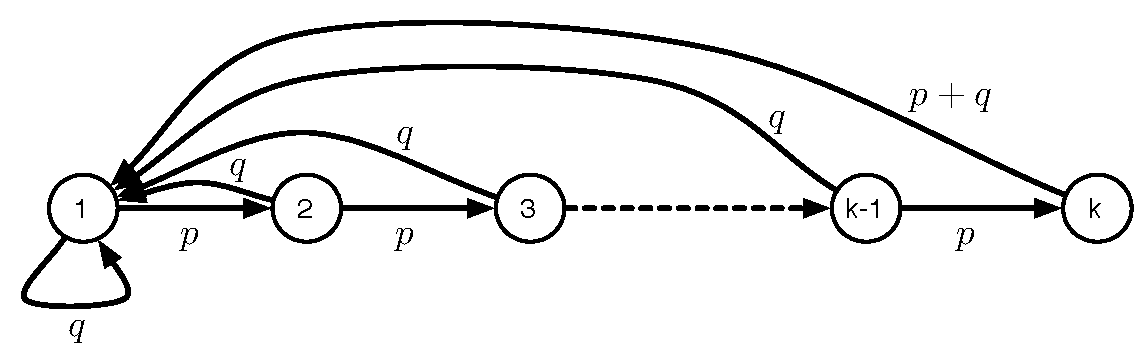
\includegraphics[width=4in]{graphics/devilsgraph.pdf} 
   %\caption{example caption}
   %\label{fig:example}
\end{figure}
Mit $T_k$ soll dieser ``Treppengraph'' bezeichnet werden''. Er hat also Knoten
(Zustände) $\{S_1,S_2,\ldots,S_k\}$ und die Kanten (Transitionen) wie
eingezeichnet.

Sie können diese grafische Darstellung 
\begin{itemize}
\item
entweder als einen endlichen Automaten (mit Startzustand $S_1$) interpretieren,
indem sie $p$ und $q$ als Symbole eines Eingabealphabets betrachten, oder
\item
als Markov-Kette betrachten, bei der die Transitionen zwischen den Zuständen
mit den Wahrscheinlichkeiten $p$ bzw. $q$ geschehen (und keine anderen als die
eingezeichneten vorkommen).
\end{itemize}

Betrachten sie zunächst die Automateninterpretation. Es bezeichne
$Ak_{i,j}^{(n)}$ die Anzahl der Pfade der Länge $n$ von $S_i$ nach $S_j$ in
$T_k$

\begin{flushenum}
\item Geben Sie explizit die Matrizen $Ak = \left[ Ak_{i,j}^{(1)} \right]$ für
	$k=2,3,4$ an und berechnen Sie deren charakteristisches Polynom.
	Welches sind die Eigenwerte?
\item Wie sehen die Matrizen $Ak$ allgemein aus, die das Geschehen in einem
	Schritt auf dieser ``Teufelsleiter'' beschreiben?\\ Zeigen Sie (z.B.
	per Induktion), dass
	\[
	\chi_{Ak}(z) = (z-2) \cdot \frac{z^k-1}{z-1}
	\]
	das charakteristische Polynom der Matrix $Ak$ ist.  Wo liegen die
	Eigenwerte der Matrix $Ak$ in der komplexen Ebene?  Machen Sie sich ein
	Bild davon!\footnote{ Bedenken Sie folgendes: das Polynom $X^k=1$ hat
	in $\mathbb{C}$ die $k$ Nullstellen $e^{2 \pi i (\ell/k)}$ für $0 \leq
	\ell < k$, genannt die (komplexen) $k$-ten Einheitswurzeln, die uns im
	Zusammenhang mit der Diskreten Fouriertransformation noch beschäftigen
	werden. Bezeichnet man mit $\omega_k$ die komplexe Zahl $e^{2 \pi i
	/k}= \cos (2 \pi/k) + i \cdot \sin(2 \pi/k)$, so sind die Nullstellen
	von $X^k=1$ gerade die Zahlen $\omega_k^\ell$ für $0 \leq \ell < k$,
	das sind die Teilungspunkte, wenn man den komplexen Einheitskreis der
	Länge $2 \pi$ in $k$ gleichlange Teile teilt, wobei $\omega_k^0=1$ ein
	Teilungspunkt ist.}
\item Betrachten Sie nun die Folgen
	\[
	\left(Ak_{1,j}^{(n)}\right)_{n \geq 0}~~\text{der Anzahlen der Pfade 
	der Länge $n$ von $S_1$ nach $S_j$ in $T_k$}
	\]
	Diese Folgen sind $C$-rekursiv und haben $\chi_{Ak}(z)$ als
	charakteristisches Polynom. \\
	Wie verhalten sich demnach die Folgen $\left(Ak_{1,j}^{(n)}\right)_{n \geq 0}$ asymptotisch 
	($n \rightarrow \infty$)? Ihre Antwort sollte die Form
	\[
	Ak_{1,j}^{(n)} \sim  \alpha_j \cdot \lambda^n
	\]
	haben. Dabei fragt sich
	\begin{itemize}
	\item Was ist $\lambda$ ? 
	\item Was ist $\alpha_j$ ?
	\end{itemize}
	Die Antwort auf die erste Frage ist einfach. \\
	Für die Antwort auf die zweite Frage bedenken Sie, dass sich aus der
	Problembeschreibung unmittelbar
	\[
	Ak_{1,j}^{(n)} = Ak_{1,j-1}^{(n-1)} ~~~(1<j\leq k)
	\]
	ergibt. Benutzen Sie das asymptotische Verhalten beider Seiten, um $2
	\alpha_j= \alpha_{j-1}$ zu folgern.  Jetzt benötigen Sie nur noch
	\begin{equation*}
		\tag{$*$} \alpha_1+\alpha_2 + \cdots + \alpha_k=1
	\end{equation*}
	um alles zu klären. Die Beziehung $(*)$ erhalten Sie, indem Sie sich
	klarmachen, was
	\[
	Ak_{1,1}^{(n)} + Ak_{1,2}^{(n)} + \cdots + Ak_{1,k}^{(n)} 
	\]
	ist und ebenfalls das asymptotische Verhalten dieser Summe betrachten.
\end{flushenum}

Im folgenden sollten Sie nun die ``stochastische'' Interpretation verwenden.
Dabei geht es um die Frage, auf welcher Stufe $S_\ell$ man den Betrunkenen nach
längerer Zeit mit welcher Wahrscheinlichkeit antrifft?

\begin{flushenum}
\setcounter{itemcounter}{3}
\item Geben Sie die (stochastischen) Matrizen $Ak(p)$ für $k=2,3,4$ explizit
	an, die diese Markovkette beschreiben und berechnen Sie deren
	charakteristisches Polynom.  Welches sind die Eigenwerte?
\item Wie sehen die Matrizen $Ak(p)$ allgemein aus, die das Geschehen in einem
	Schritt auf dieser ``Teufelsleiter''  beschreiben?\\ Zeigen Sie (z.B.
	per Induktion), dass
	\[
	\chi_{Ak(p)}(z) = (z-1) \cdot \frac{z^k-p^k}{z-p}
	\]
	das charakteristische Polynom der Matrix $Ak(p)$ ist.  Wo liegen die
	Eigenwerte der Matrix $Ak(p)$ in der komplexen Ebene?  Machen Sie sich
	ein Bild davon!

\item Es bezeichne nun $\mathtt{P}_\ell^{(n)}$ die Wahrscheinlichkeit, dass der
	Betrunkene nach $n$ Schritten auf der Stufe $S_\ell$ anzutreffen ist.
	Teil 5 der Aufgabe besagt insbesondere, dass $\lambda=1$ ein dominanter
	Eigenwert der Matrix $Ak(p)$ ist.
	Daher gibt es eine eindeutig bestimmte stationäre
	Wahrscheinlichkeitsverteilung $\boldsymbol{\pi}=(\pi_j)_{1 \leq j \leq
	k}$ auf der Menge $\{S_j\,;\, 1 \leq j \leq k\}$  der Zustände und es
	gilt
	\[
	\lim_{n \rightarrow \infty} \mathtt{P}_j^{(n)} = \pi_j ~~~(1 \leq j \leq k).
	\]
	Bestimmen Sie $(\pi_j)_{1 \leq j \leq k}$, indem sie die Beziehung
	\[
	\mathtt{P}_j^{(n)} = \mathtt{P}_{j-1}^{(n-1)} \cdot p~~~(1<j\leq k)
	\]
	und das asymptotische Verhalten verwenden --- ganz analog wie in Teil 3
	dieser Aufgabe.
\end{flushenum}

Hinweis: Das Ganze hat etwas mit einer endlichen geometrischen Reihe zu tun.
Schauen Sie in Kapitel 1 nach, falls Sie vergessen haben, was es damit auf sich
hat.


%%%
% Lösung
%%%
\subsection*{Lösung}
\begin{flushenum}
% teil 1: automaten interpretation, Ak für k = 2,3,4
\item
	\begin{itemize}
		\item $k= 2$: 
			\[ A2 = \begin{bmatrix}
					1 & 1 \\
					2 & 0 \\
				\end{bmatrix} \]
			\[ \chi_2(z) = 
				\begin{vmatrix}
					z - 1 & -1 \\
					-2    & z  \\
				\end{vmatrix} =
				z^2 - z - 2 = (z-2)(z+1) \]
			Die Eigenwerte sind $\lambda_1 = 2$ und $\lambda_2 = -1$.
		\item $k = 3$:
			\[ A3 = \begin{bmatrix}
					1 & 1 & 0 \\
					1 & 0 & 1 \\
					2 & 0 & 0 \\
				\end{bmatrix} \]
			\[ \chi_3(z) = 
				\begin{vmatrix}
					z-1 & -1 & 0 \\
					-1 & z & -1 \\
					-2 & 0 & z \\
				\end{vmatrix} =
				z^3 - z^2 - z - 2 = (z-2)(z^2 + z + 1) \]
			Die Eigenwerte sind $\lambda_1 = 2, \lambda_2 = \omega_3, \lambda_3 = \omega_3^2 $,
			wobei $\omega_3$ die dritte Einheitswurzel $e^{\imath 2 \pi / 3}$ ist.
		\item $k = 4$:
			\[ A4 =	\begin{bmatrix}
					1 & 1 & 0 & 0 \\
					1 & 0 & 1 & 0 \\
					1 & 0 & 0 & 1 \\
					2 & 0 & 0 & 0 \\
				\end{bmatrix} \]
			\[ \chi_4(z) = 
				\begin{vmatrix}
					z-1 & -1 & 0 & 0 \\
					-1 & z & -1 & 0 \\
					-1 & 0 & z & -1 \\
					-2 & 0 & 0 & z \\
				\end{vmatrix} = 
				(z-1) z^3 + 
					\begin{vmatrix}
						-1 & -1 & 0 \\
						-1 & z & -1 \\
						-2 & 0 & z \\
					\end{vmatrix} = \] \[
				(z-1)z^3 - z^2 - z  - 2 =
				z^4 - z^3 - z^2 - z - 2 =
				(z-2)(z^3 + z^2 + z + 1) \]
			Die Eigenwerte sind $\lambda_1 = 2, \lambda_2 = \omega_4, \lambda_3 = \omega_4^2, \lambda_4 = \omega_4^3$,
			wobei $\omega_4$ die vierte Einheitswurzel $e^{\imath 2 \pi / 4} = \imath$ ist.
	\end{itemize}

% teil 2: allgemeine Ak
\item Allgemein sieht die Matrix $Ak$ folgendermaßen aus:
	\[ Ak = \begin{bmatrix}
			1      & 1      & 0      & \cdots & 0      \\
			1      & 0      & 1      &        & \vdots \\
			\vdots & \vdots & \ddots & \ddots & 0      \\
			1      & \vdots &        & \ddots & 1      \\
			2      & 0      & \cdots & \cdots & 0      \\
		\end{bmatrix} \]
	Das Charakteristische Polynom lässt sich rekursiv berechnen (Entwicklung nach erster Zeile,
	nachdem 2. Spalte auf 1. Spalte addiert wurde):
	\begin{eqnarray*}
		\chi_k(z) & = &
				\begin{vmatrix}
					z-1    & -1     & 0      & \cdots & \cdots & 0      \\
					-1     & z      & \ddots & \ddots &        & \vdots \\
					\vdots & 0      & \ddots & \ddots & \ddots & \vdots \\
					\vdots & \vdots & \ddots & \ddots & \ddots & 0      \\
					-1     & \vdots &        & \ddots & \ddots & -1     \\
					-2     & 0      & \cdots & \cdots & 0      & z      \\
				\end{vmatrix} = %\\[2em]
				%& \hspace{\0.3\linewidth} =
				\begin{vmatrix}
					z-2    & -1     & 0      & \cdots & \cdots & 0      \\
					z-1    & z      & \ddots & \ddots &        & \vdots \\
					-1     & 0      & \ddots & \ddots & \ddots & \vdots \\
					\vdots & \vdots & \ddots & \ddots & \ddots & 0      \\
					-1     & \vdots &        & \ddots & \ddots & -1     \\
					-2     & 0      & \cdots & \cdots & 0      & z      \\
				\end{vmatrix} = \\%\displaybreak \\
			& = & (z-2) \cdot
				\begin{vmatrix}
					& z      & -1     & 0      & \cdots & 0      \\
					& 0      & \ddots & \ddots & \ddots & \vdots \\
					& \vdots & \ddots & \ddots & \ddots & 0      \\
					& \vdots &        & \ddots & \ddots & -1     \\
					& 0      & \cdots & \cdots & 0      & z      \\
				\end{vmatrix} +
				\begin{vmatrix}
					z-1    & -1     & 0      & \cdots & 0      \\
					-1     & z      & \ddots & \ddots & \vdots \\
					\vdots & 0      & \ddots & \ddots & 0      \\
					-1     & \vdots & \ddots & \ddots & -1     \\
					-2     & 0      & \cdots & 0      & z      \\
				\end{vmatrix} = \\%\\[1.5em]
			&=& (z-2) z^{k-1} + \chi_{k-1}(z)
	\end{eqnarray*}
	Mit Hilfe dieses Zusammenhangs kann man per vollständiger Induktion die gewünschte Formel beweisen:
	\begin{itemize}
		\item \textit{I.A.}: $k=2$: \[ \chi_2(z) = (z-2)(z+1) = (z-2)\frac{(z+1)(z-1)}{z-1} = (z-2)\frac{z^2 - 1}{z-1} \]
		\item \textit{I.V.}: Für ein $k \in \mathbb{N}$ gelte:
			\[ \chi_k(z) = (z-2)\frac{z^k - 1}{z-1} \]
		\item \textit{I.S.}: $k \rightarrow k+1$:
			\begin{eqnarray*}
			\chi_{k+1}(z) &=& (z-2) z^{k} + \chi_k(z) \overset{I.V.}{=} (z-2) z^k + (z-2) \frac{z^k - 1}{z-1} \\
			   &=& (z-2) \frac{z^k (z-1)}{z-1} + (z-2)\frac{z^k - 1}{z-1} =
			   (z-2) \frac{z^{k+1} - 1}{z-1}
			\end{eqnarray*}
	\end{itemize}
	Die Eigenwerte sind zum einen $\lambda_1 = 2$ und zum anderen die Lösungen von $z^k - 1 = 0$ (außer $z = 1$), also den
	$k$-ten Einheitswurzeln, $\lambda_i = e^{\imath 2 \pi \frac{j}{k}}$ mit $1 \leq j \leq k-1$, sie liegen
	auf einem Kreis mit Radius $1$ um den Ursprung.

\item 
Da die Folgen $\left( Ak_{1,j}^{(n)} \right)_{n \geq 0}$ C-Rekursionen sind, die das charakteristische Polynom $\chi_k(z)$
aus der vorigen Aufgabe haben ist der dominante Eigenwert $\lambda = \lambda_1 = 2$.
Aus der Problembeschreibung ergibt sich 
\[ Ak_{1,j}^{(n)} = Ak_{1,j-1}^{(n-1)} \quad \quad (1 < j \leq k) \]
da der Betrunkene erst auf der Stufe $j-1$ nach $n-1$ Schritten gewesen sein muss, wenn er Stufe $j$ nach $n$ Schritten erreichen will.
Auf Grund der Asymptotik ergibt sich somit:
\[ Ak_{1,j}^{(n)} = \alpha_j \cdot 2^n = Ak_{1,j-1}^{(n-1)} = \alpha_{j-1} \cdot 2^{n-1} \quad \quad (1 < j \leq k) \]
also $2 \cdot \alpha_j = \alpha_{j-1}$.

\[ Ak_{1,1}^{(n)} + Ak_{1,2}^{(n)} + \ldots + Ak_{1,k}^{(n)} = \alpha_1 \cdot 2^n + \alpha_2 \cdot 2^n + \ldots + \alpha_k \cdot 2^n = 2^n \]
ist die Summe aller Pfade der Länge $n$ in dem Graphen, die bei $1$ beginnen und auf einer beliebigen Stufe zwischen $1$ und $k$ enden.
Da der Graph einen Automaten beschreibt, der in jedem Zustand zwei Eingabewerte ($p$ und $q$) akzeptiert, sind dies offensichtlich
$2^n$ mögliche Pfade.
Somit folgt (*) $\alpha_1 + \alpha_2 + \ldots + \alpha_k = 1$.
Mit $2 \cdot \alpha_j = \alpha_{j-1} $ erhält man weiterhin 
\[ \alpha_1 + \alpha_2 + \ldots + \alpha_k = \alpha_1 \sum_{j=0}^{k-1} \left( \frac{1}{2}\right)^j 
   = \alpha_1  \frac{1 - \left(\frac{1}{2}\right)^k}{1 - \frac{1}{2}}  = 1 \]
Folglich ist 
\[ \alpha_1 = \frac{1}{\left(\frac{1}{2}\right)^{k-1} - 2} = \frac{2^{k-1}}{2^k - 1} \]
\[ \alpha_j = \left(\frac{1}{2}\right)^{j-1} \cdot \alpha_1 = \frac{2^{k-j}}{2^k - 1}\]

\item
  $A_{k,p}$ für $k = 2, 3, 4$:

  \begin{minipage}{0.4\linewidth}
  \[ A_{2,p} = \begin{bmatrix} 1-p & p \\ 1 & 0 \end{bmatrix} \]
  \[ \chi_{2,p}(z) = \begin{vmatrix} 1-p-z & p \\ 1 & -z \end{vmatrix} \]
  \[ = z^{2} + pz - z - p \]
  \[ \lambda_{1} = 1, \quad \lambda_{2}= -p \]
  \vspace{0.5em}
  \[ A_{3,p} = \begin{bmatrix} 1-p & p & 0 \\
                               1-p & 0 & p \\
                                 1 & 0 & 0 \end{bmatrix} \]
  \[ \chi_{3,p}(z) = \begin{vmatrix} 1-p-z & p  & 0 \\
                                       1-p   & -z & p \\
                                       1     & 0  & -z \end{vmatrix} \]
  \[ = -z^{3} - pz^{2} + z^{2} - p^{2}z + pz + p^{2} = \]
  \[ = -(z - 1) (z^{2} + pz + p^{2}) \]
  \[ \lambda_{1}= 1 \]
  \[ \lambda_{2/3}= -\frac{p}{2}(1 \pm i\sqrt{3}) \]
  \end{minipage}\hfill\begin{minipage}{0.5\linewidth}
  \[ A_{4,p} = \begin{bmatrix} 1-p & p & 0 & 0 \\
                               1-p & 0 & p & 0 \\
                               1-p & 0 & 0 & p \\
                                 1 & 0 & 0 & 0 \end{bmatrix} \]
  \[ \chi_{4,p}(z) = det(A_{4,p} - z\cdot \mathds{1}) = \]
  \[                 -\begin{vmatrix} p & 0 & 0 \\
                                     -z & p & 0 \\
                                      0 &-z & p \end{vmatrix} 
                     -\begin{vmatrix} 1-p-z & p & 0 \\
                                      1-p & -z & p \\
                                      1-p & 0 & -z \end{vmatrix} \]
  \[ = z^4 + pz^3 - z^3 + p^{2}z^2 - pz^2 + p^{3}z - p^{2}z -p^3 \]
  \[ = (z - 1) (z^{3} + pz^{2} + p^{2}z + p^{3}) \]
  \[ \lambda_{1}= 1, \]
  \[ \lambda_{2}= -p, \quad
     \lambda_{3}= ip, \quad
     \lambda_{4}= -ip\]
  \end{minipage}
  
\item
  \[ A_{k,p} = \left[a_{ij}\right]_{1\leq i,j\leq k}, \]
  \[ a_{ij} = \begin{cases} 1-p &\text{wenn~} j = 0, i \not= k \\
                              1 &\text{wenn~} j = 0, i = k \\
                              p &\text{wenn~} j = i + 1 \\
                              0 &\text{sonst} \end{cases} \]

  zu zeigen: \[ \chi_{k,p}(z) = (z - 1) \frac{z^{k}-p^{k}}{z-p}(-1)^{k} \]
  Beweis durch Induktion über $k$.
  \begin{itemize}
    \item \textit{I.A.}: $k = 2$
      \[ \chi_{z,p}(z) = (z - 1) \frac{z^{2}-p^{2}}{z-p} = (z-1)(z+p) \]
    \item \textit{I.V.}: Die Behauptung gelte für $k$.
    \item \textit{I.S.}: $k \rightarrow k + 1$

      Addition der zweiten auf die erste Spalte:
      \begin{equation*}
      \begin{split} \chi_{A_{k}}(z) & = \begin{vmatrix}
                            1-p-z & p  & 0  & \cdots & \cdots & 0 \\
                            1-p & -z & p  & \ddots & \ddots & \vdots \\
                            \vdots & 0  & \ddots & \ddots & \ddots & \vdots \\
                            \vdots & \vdots  & \ddots & \ddots & \ddots & 0 \\
                            1-p & \vdots  & \ddots & \ddots & \ddots & p \\
                            1 & 0 & \cdots & \cdots & 0 & -z
                           \end{vmatrix} \\
                       & = \begin{vmatrix}
                            1-z & p  & 0  & \cdots & \cdots & 0 \\
                            1-p-z & -z & p  & \ddots & \ddots &\vdots \\
                            1-p & 0  & \ddots & \ddots & \ddots & \vdots \\
                            \vdots & \vdots  & \ddots & \ddots & \ddots & 0 \\
                            1-p & \vdots  & \ddots & \ddots & \ddots & p \\
                            1 & 0 & \cdots & \cdots & 0 & -z
                           \end{vmatrix} = \\
       & = -(z - 1) (-z)^{k-1} - p\chi_{A_{k-1}}(z) = \\
       & = (-1)^{k}(z - 1) z^{k-1} - p(z-1)\frac{z^{k-1}-p^{k-1}}{z-p} = \\
       & = (-1)^{k}(z - 1) \left( z^{k-1} + \frac{pz^{k-1}-p^{k}}{z-p} \right) = \\
       & = (-1)^{k}(z - 1) \left( \frac{z^{k}-z^{k-1}p}{z-p} +
                          \frac{pz^{k-1}-p^{k}}{z-p} \right) = \\
       & = (-1)^{k}(z - 1) \left( \frac{z^{k}-p^{k}}{z-p} \right)
       \end{split}
       \end{equation*}

      $\chi_{A_{k,p}}$ hat die Nullstellen $1$ und die $k$-ten Wurzeln von
      $p^{k}$, welche in der komplexen Ebene auf einem Kreis mit Radius $p$ um
      den Ursprung liegen.
  \end{itemize}

%\item
%  Da man die Stufe $S_{l}$ nur auf direktem Weg in $l - 1$ Schritten erreichen
%  kann, muss man, um beim $n$-ten Schritt auf Stufe $S_{l}$ zu landen, zuvor
%  nach $n - l - 1$ Schritten auf der ersten Stufe gestanden haben.
%
%  Die Wahrscheinlichkeit ergibt sich aus dem Produkt der
%  Einzelwahrscheinlichkeiten.

  \item
   \[ \lim_{n\rightarrow\infty} P_{1}^{(n)} = a, \quad
      1 = \sum_{i=1}^{k} a \cdot p^{l-1} = \sum_{i=0}^{k-1} a \cdot p^{l} = a
   \sum_{l=0}^{k-1} p^{l} = a \frac{1-p^{k}}{1-p} \]
  \[ \Rightarrow a = \frac{1-p}{1-p^{k}} \]

  \[ (\pi_{i})_{1\leq l\leq k} = (a\cdot p^{l-1})_{1\leq l\leq k} 
     = (\frac{p^{l-1} - p^{l}}{1-p^{k}})_{1\leq l\leq k} \]
\end{flushenum}

\section*{Aufgabe 17 - inhomogene Rekursion}
\addcontentsline{toc}{subsection}{Aufgabe 17 - inhomogene Rekursion}
\[ x_{n} = 4x_{n-1} - 4x_{n-2} + f_{n} \quad (n\geq 2) \]
\begin{flushenum}
\item
  Lösungen der homogenen Rekursion
  \[ x_{n} = 4x_{n-1} - 4x_{n-2} \]
  \[ \chi(z) = z^{2} - 4z + 4 = (z - 2)^{2} \]
  also der doppelte Eigenwert
  \[ \lambda = 2 \]
  und damit
  \[ x_{n} = \alpha_{1}2^{n} + \alpha_{2}n2^{n} \]

  \[ \textnormal{für } \alpha_{2} = 0 \Rightarrow x_{n} \sim \alpha_{1}2^{n} \]
  \[ \textnormal{für } \alpha_{2} \not= 0 \Rightarrow x_{n} \sim \alpha_{2}n2^{n} \]
  \[ \textnormal{für } x_{0} = x_{1} = 0 \Rightarrow x_{n} = 0 \]
\item
  spezielle Lösungen der inhomogenen Rekursion
  \begin{enumerate}[(a)]
    \item $f = (1, 1, \dots) = (1^{n})_{n\geq 0}$
      \[ x_{n} = 4x_{n-1} - 4x_{n-2} + 1^{n} \]
      \[ x_{n+1} = 4x_{n} - 4x_{n-1} + 1^{n+1} \]

      \[ x_{n} - x_{n+1} = 4x_{n-1} - 4x_{n-2} - 4x_{n} + 4x_{n-1} \]
      \[ -x_{n+1} = -5x_{n} + 8x_{n-1} - 4x_{n-2} \]
      \[ x_{n} = 5x_{n-1} - 8x_{n-2} + 4x_{n-3} \]

      \[ \chi(z) = z^{3} - 5z^{2} + 8z -  4 = (z - 1) (z - 2)^{2} \]
      \[ \lambda_{1} = 1, \lambda_{2} = 2 \textnormal{ (doppelter EW)} \]

      \[ x_{n} = \alpha_{1}1^{n} + \alpha_{2}2^{n} + \alpha_{3}n2^{n} \]
      Durch einsetzen in die ursprüngliche Rekursion erhält man $\alpha_{1} =
      1$ und damit
      \[ x_{n} = 1 + \alpha 2^{n} + \beta n2^{n} \]
    \item $f = (1, 2, 4, \dots) = (2^{n})_{n\geq 0}$
      \[ x_{n} = 4x_{n-1} - 4x_{n-2} + 2^{n} \]
      \[ x_{n+1} = 4x_{n} - 4x_{n-1} + 2^{n+1} \]

      \[ 2x_{n} - x_{n+1} = 8x_{n-1} - 8x_{n-2} - 4x_{n} + 4x_{n-1} \]
      \[ -x_{n+1} = -6x_{n} + 12x_{n-1} - 8x_{n-2} \]
      \[ x_{n} = 6x_{n-1} - 12x_{n-2} + 8x_{n-3} \]

      \[ \chi(z) = z^{3} - 6z^{2} + 12z - 8 = (z - 2)^{3} \]
      \[ \lambda = 2, \textnormal{ (dreifacher EW)} \]

      \[ x_{n} = \alpha_{1}2^{n} + \alpha_{2}n2^{n} + \alpha_{3}n^{2}2^{n} \]
      Durch einsetzen in die ursprüngliche Rekursion erhält man wiederum
      $\alpha_{3} = \frac{1}{2}$ und damit
      \[ x_{n} = \alpha_1 2^{n} + \alpha_2 n2^{n} + n^{2}2^{n-1}\]
    \item $f = (1, 3, 9, \dots) = (3^{n})_{n\geq 0}$
      \[ x_{n} = 4x_{n-1} - 4x_{n-2} + 3^{n} \]
      \[ x_{n+1} = 4x_{n} - 4x_{n-1} + 3^{n+1} \]

      \[ 3x_{n} - x_{n+1} = 12x_{n-1} - 12x_{n-2} - 4x_{n} + 4x_{n-1} \]
      \[ -x_{n+1} = -7x_{n} + 16x_{n-1} - 12x_{n-2} \]
      \[ x_{n} = 7x_{n-1} - 16x_{n-2} + 12x_{n-3} \]

      \[ \chi(z) = z^{3} - 7z^{2} + 16z - 12 = (z - 3) (z - 2)^{2} \]
      \[ \lambda_{1} = 3, \lambda_{2} = 2, \textnormal{ (doppelter EW)} \]

      \[ x_{n} = \alpha_{1}3^{n} + \alpha_{2}2^{n} + \alpha_{3}n2^{n} \]
      Erneut wird durch Einsetzen in die ursprüngliche Rekursionsgleichung der
      Parameter $\alpha_{1} = 9$ eliminiert und es ergibt sich
      \[ x_{n} = \alpha 2^{n} + \beta n2^{n} + 3^{n+2} \]
  \end{enumerate}
  \begin{paragraph}{Asymptotisches Verhalten}
    \begin{enumerate}[(a)]
      \item \[ x_{n} = 1 + \alpha 2^{n} + \beta n2^{n} \]
        \begin{equation*}
          \begin{split}
           \beta \not= 0 &\quad x_{n} \sim \beta n2^{n} \\
           \beta = 0, \alpha \not= 0 &\quad x_{n} \sim \alpha 2^{n} \\
           \beta = \alpha = 0 & \quad x_{n} = 1
          \end{split}
        \end{equation*}
      \item \[ x_{n} = \alpha2^{n} + \beta n2^{n} + n^{2}2^{n-1}\]
        \[ x_{n} \sim n^{2}2^{n-1} \]
      \item \[ x_{n} = \alpha 2^{n} + \beta n2^{n} + 3^{n+2} \]
        \[ x_{n} \sim 3^{n+2} \]
    \end{enumerate}
  \end{paragraph}
  \begin{paragraph}{Alternative Lösung}
	Alternativ lässt sich diese Aufgabe auch durch Überlegungen aus dem
	Skript lösen:
	\[ x_{n} = 4x_{n-1} - 4x_{n-2} + y_{n} \]
	Ist die Folge $(y_n)_{n\geq 0}$ ebenfalls C-rekursiv, so genügt die
	Folge $(x_n)_{n\geq 0}$ einer homogenen Rekursion mit
	charakteristischem Polynom $\chi_x(z)\cdot\chi_y(z)$ (Skript S. 83).

	Das charakteristische Polynom von $(y_n)_{n\geq 0}$ erhält man
	beispielsweise über die Rei\-hen\-ent\-wicklung der $z$-Transformierten
	\[ y(z) = \sum_{n\geq 0} y_n z^n = \frac{c(z)}{d(z)}. \]
	Das Polynom $d(z)$ entspricht dabei dem \textit{Rekursionspolynom} zu
	$(y_n)_{n\geq 0}$, aus dem sich unmittelbar das charakteristische
	Polynom ableiten lässt.

	Die resultierende Rekursion entspricht genau der homogenen Rekursion,
	die in \textbf{2.} durch Eliminierung des inhomogenen Terms entstand.
	Nachdem die Eigenwerte dieser Rekursion bestimmt sind verfährt man wie
	bisher.
  \end{paragraph}
\end{flushenum}

\end{document}
